\subsection{Simulation with simulink}

A simulation were done in  simulink  to  compare the tracking behavior between
simulation and  experiment.  The best value for the $PT_{1}$ we determine were
$5.947$ so our $PT_{1}$ element is from the form:

\begin{equation}
    G(s) = \frac{1}{5.947s+1}
\end{equation}

For   the   dead  time  element  we  took   the   value   $0.0750$.   In   the
\ref{fig:simulink} there are 5 different Block diagram.  the  first  3 diagram
represent  the  simulation  model  of  the  plant. The last two Block Diagramm
represent an implemented PID controller  with and without a tracking behavior.

\begin{figure}
    \centering
    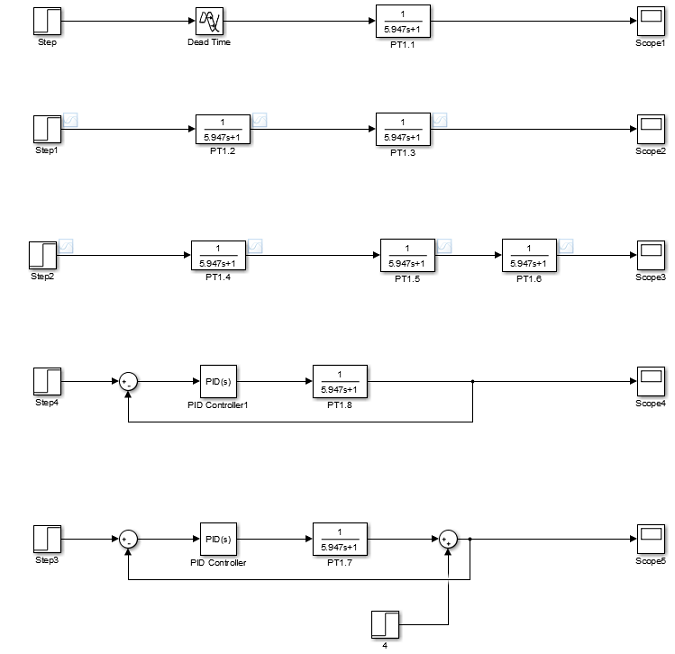
\includegraphics[width=\imagewidth]{images/simulink.png}
    \caption{Block diagram of the Simulink simulation}
    \label{fig:simulink}
\end{figure}

Unfortunately  the  time in the  laboratory  was  not  enough  to  finish  the
exercise. So we don't had the time to analyse  the  tracking  behavior  of the
electrical motor in the laboratory. However, in Simulink the tracking behavior
were analysed and it can be seen in \ref{fig:tracking}.

\begin{figure}
    \centering
    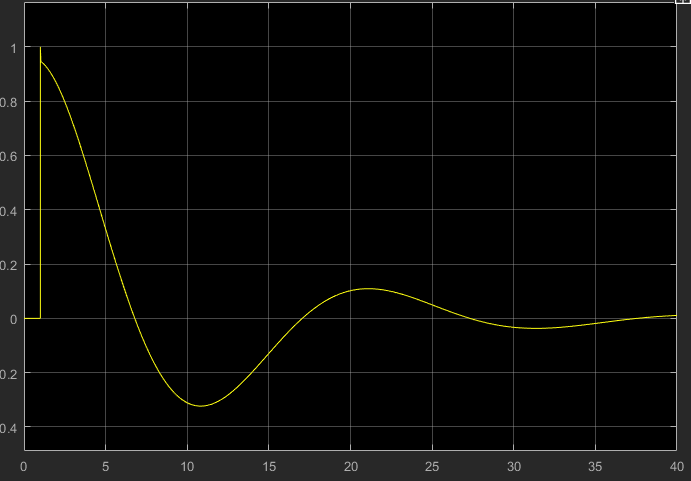
\includegraphics[width=\imagewidth]{images/slope_tracking.png}
    \caption{Tracking behavior of the system}
    \label{fig:tracking}
\end{figure}

